\documentclass[twocolumn,10pt]{article}

\usepackage{authblk}
\usepackage{bera}
\usepackage[utf8]{inputenc}
\usepackage{graphicx}
\usepackage{booktabs}

% TITLE
\title{Chef Classification Task - NLP Project}

% AUTHORS
\author{João Lopes}
\author{Kun Fang}
\author{Tomás Henriques}
\author{Tomás Cruz}
\affil{Group 64\\ Instituto Superior Técnico, Universidade de Lisboa}

\begin{document}

\maketitle

\section{Introduction}

The task addressed in this project is a multi-class classification problem. The goal is to assign each recipe to one of six chefs using features extracted from recipe name, tags, steps, description, and ingredients. The dataset contains a total of 2,999 recipes with moderate class imbalance (percentages per chef: 13.47\%, 15.04\%, 26.88\%, 17.81\%, 12.40\%, 14.40\%, respectively). The challenge lies in distinguishing recipes that may share similar ingredients or steps, requiring models that can capture subtle textual differences.  

\section{Models}

Two main approaches were explored: a recurrent neural network (RNN) and a linear support vector classifier (LinearSVC).  

\subsection{Preprocessing}
For LinearSVC, all textual fields were concatenated, lowercased, tokenized, and transformed into TF-IDF features using unigrams and bigrams. Stopwords were removed to reduce noise. For the RNN, fields were concatenated and tokenized, with no removal of stopwords, to preserve sequential information. No data augmentation was applied.  

\subsection{Model Architecture}
The RNN used an embedding layer of 128 dimensions, a bidirectional LSTM with hidden size 128, a dropout rate of 0.3, and sequences truncated or padded to a maximum length of 100 tokens. LinearSVC was used with optimized hyperparameters obtained via GridSearchCV on a subset of the training data.  

\section{Experimental Setup}

\subsection{Datasets}
The original dataset was split into training and testing sets using four different ratios: 0.5, 0.7, 0.8, and 0.9. For each split, the dataset was shuffled to avoid repeating the same training/testing distribution.  

\subsection{Evaluation Metrics}
Accuracy, macro F1-score, and weighted F1-score were used to evaluate model performance. Confusion matrices were also generated to assess per-class performance and to analyze common misclassifications.  

\subsection{Hyperparameters}
The best hyperparameters for the RNN were: hidden\_dim = 128, embed\_dim = 128, dropout = 0.3, training epochs = 30, and MAX\_LEN = 100. LinearSVC used: C = 2.0, TF-IDF max\_df = 1.0, min\_df = 2, ngram\_range = (1, 2).  

\section{Results}

Table~\ref{tab:results_summary} summarizes the accuracy and F1-scores for RNN and LinearSVC across different splits. LinearSVC consistently outperformed the RNN, reaching up to 95.33\% accuracy on the 0.9 split, while RNN peaked at 65.67\%.  

\begin{table}[h!]
\centering
\caption{Model Performance by Split Ratio}
\label{tab:results_summary}
\begin{tabular}{lccc}
\toprule
Split & Model & Accuracy & F1-macro \\
\midrule
0.5 & RNN & 0.5433 & 0.5205 \\
0.5 & LinearSVC & 0.9207 & 0.9108 \\
0.7 & RNN & 0.6311 & 0.6161 \\
0.7 & LinearSVC & 0.9367 & 0.9283 \\
0.8 & RNN & 0.6133 & 0.5939 \\
0.8 & LinearSVC & 0.9400 & 0.9311 \\
0.9 & RNN & 0.6567 & 0.6399 \\
0.9 & LinearSVC & 0.9533 & 0.9469 \\
\bottomrule
\end{tabular}
\end{table}

\subsection{Confusion Matrix Analysis}
Figure~\ref{fig:confusion_svc} shows the confusion matrix for LinearSVC with split 0.8. Most misclassifications occur for chefs with fewer samples, such as 1533 and 3288, reflecting the moderate imbalance in the dataset. The RNN confusion matrices show more distributed errors across classes, indicating difficulty in learning distinguishing features from sequential information.  

\begin{figure}[h!]
\centering
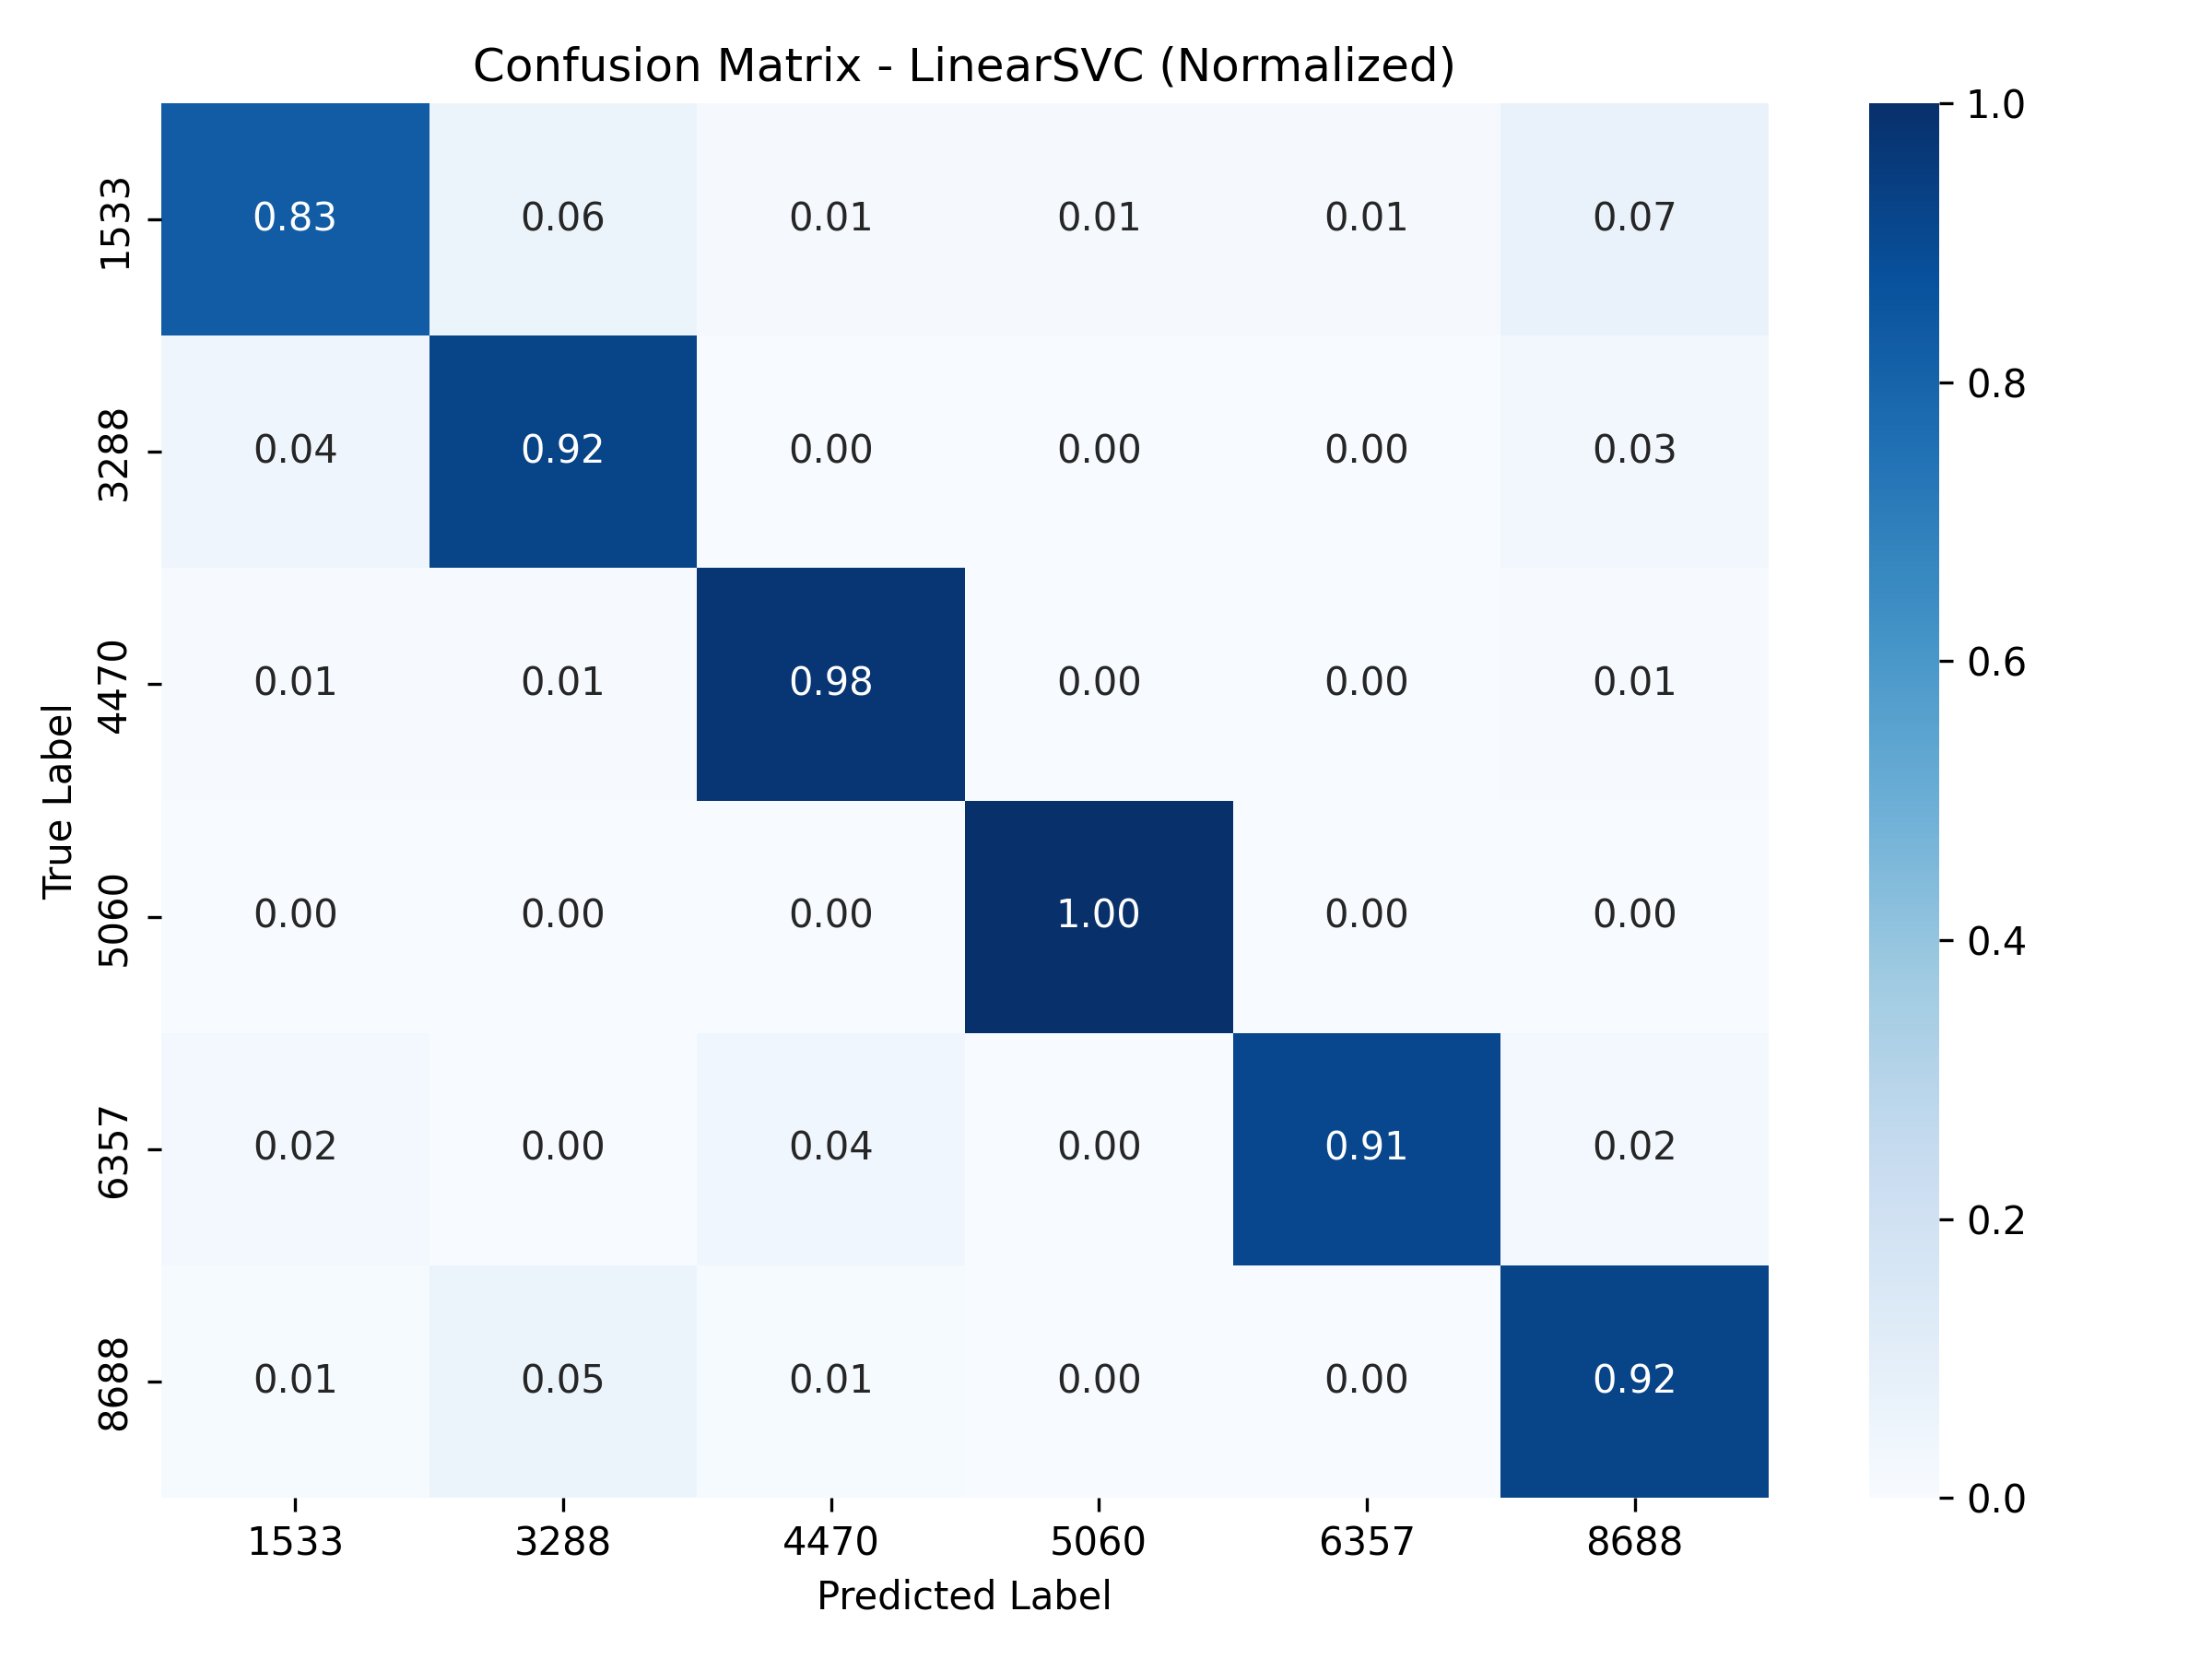
\includegraphics[width=\linewidth]{confusion_matrix_svc.png}
\caption{Confusion matrix of LinearSVC on split 0.8. Rows correspond to true labels, columns to predicted labels.}
\label{fig:confusion_svc}
\end{figure}

\section{Discussion}

The LinearSVC consistently outperformed the RNN across all splits. This result can be attributed to the nature of the dataset: distinguishing features are largely captured by word occurrence and frequency rather than sequence, favoring bag-of-words approaches. The RNN struggled, likely due to insufficient data to learn meaningful sequential patterns for six classes.  

Errors identified in the confusion matrices mainly involve chefs with fewer recipes (1533 and 6357), consistent with the moderate class imbalance (13–27\%). The RNN frequently misclassified recipes between chefs with overlapping vocabulary in ingredients and steps, while LinearSVC effectively separated classes using TF-IDF weighted word features.  

\section{Future Work}

Improvements could include:  

\begin{itemize}
    \item Applying data augmentation techniques such as synonym replacement or recipe paraphrasing to increase training data diversity.  
    \item Experimenting with pre-trained embeddings or transformer-based models, which may better capture contextual relationships in text.  
    \item Implementing class weighting or oversampling to address moderate imbalance.  
    \item Performing hyperparameter optimization for RNN depth, hidden size, and learning rate to potentially improve sequential learning.  
\end{itemize}

\section*{Bibliography}

\bibliographystyle{apalike}
\bibliography{biblio}

\appendix

\section*{Appendix A: Additional Figures and Tables}

\begin{table}[h!]
\centering
\caption{Percentage of Recipes per Chef}
\begin{tabular}{lcc}
\toprule
Chef ID & Count & Percentage (\%) \\
\midrule
1533 & 404 & 13.47 \\
3288 & 451 & 15.04 \\
4470 & 806 & 26.88 \\
5060 & 534 & 17.81 \\
6357 & 372 & 12.40 \\
8688 & 432 & 14.40 \\
\bottomrule
\end{tabular}
\end{table}

\end{document}
